\documentclass[conference]{IEEEtran}
\usepackage{cite}
\usepackage{amsmath,amssymb}
\usepackage{graphicx}
\usepackage{booktabs}
\usepackage{xcolor}
\usepackage{url}
\usepackage{tikz}
\usetikzlibrary{arrows.meta,positioning,shapes.geometric}
\usepackage[hidelinks]{hyperref}
\hypersetup{
  colorlinks=true,
  linkcolor=blue,
  citecolor=blue,
  urlcolor=blue,
  pdfauthor={P. Deepesh Reddy, R. Vignesh, R. Sidhardh Reddy, Saharsh Machendra, V. Surya Venkat, K. Vishal Reddy},
  pdftitle={X-Fusion: A Tri-Modal Transformer System for Multi-Label Chest X-ray Screening}
}

\begin{document}

\title{X-Fusion: A Tri-Modal Transformer System for Multi-Label Chest X-ray Screening}

\author{\IEEEauthorblockN{P. Deepesh Reddy, R. Vignesh, R. Sidhardh Reddy, Saharsh Machendra, V. Surya Venkat, and K. Vishal Reddy}
\IEEEauthorblockA{Department of Computer Science and Engineering\\
Keshav Memorial Institute of Technology\\
Hyderabad, Telangana, India\\
Email: \texttt{Kasarlavishalreddy@gmail.com}}}

\maketitle

\begin{abstract}
Chest radiographs are read in the context of a patient's history and measurements, but many automated systems still consider the image alone. We describe X-Fusion, a research prototype that accepts a radiograph, a clinical note, and six patient fields: age, sex, temperature, heart rate, respiratory rate, and oxygen saturation. Its image, text, and metadata encoders feed a two-layer Transformer, which combines one representation from each modality with a learned classification token. A fourteen-output sigmoid head produces scores for the selected findings. The prototype also includes a FastAPI service, a Next.js interface, an attention visualization, and aggregate Kernel SHAP metadata attributions. In a saved 14-epoch run, training-objective loss decreased from 0.1545 to 0.1190, while validation classification loss decreased from 0.0207 to 0.0007. These values describe optimization, not diagnostic performance: the current data pipeline generates notes and several vital signs from disease labels, introducing target leakage. We therefore report software and training observations rather than clinically validated results.
\end{abstract}

\begin{IEEEkeywords}
Chest radiography, multimodal learning, Vision Transformer, medical NLP, multi-label classification, explainable AI, clinical decision support.
\end{IEEEkeywords}

\section{Introduction}
Chest radiographs are routinely used to assess pulmonary and cardiothoracic conditions. Deep learning models have been trained to classify findings in large collections such as NIH ChestX-ray14 and CheXpert \cite{wang2017,irvin2019}. Vision Transformers represent an image as a sequence of patches and use self-attention to capture relationships between them \cite{dosovitskiy2021}. Biomedical image and language encoders provide pretrained representations that can be adapted to related tasks \cite{biomedclip2023,cxrbert2022}.

An image is only one part of the information considered during screening. Symptoms, the reason for imaging, demographic information, and vital signs may also inform interpretation. X-Fusion was built to demonstrate a workflow that brings these inputs together: a web application collects them, a Python service runs the model, and the interface displays finding scores with visual explanations.

This paper documents the implemented prototype: three modality encoders, a compact Transformer fusion stage, a fourteen-label output head, an API, and a browser interface. It is important to distinguish that engineering work from clinical validation. In the current data pipeline, generated reports and several synthetic vital signs are derived from the target labels. As a result, predictive metrics from the checkpoint would not provide reliable evidence of clinical performance.

\section{Related Work}
\subsection{Chest X-ray Classification}
NIH ChestX-ray14 introduced a large-scale collection of chest radiographs with fourteen finding labels \cite{wang2017}. CheXpert provides chest radiographs and report-derived labels with uncertainty categories, alongside a radiologist-annotated evaluation subset \cite{irvin2019}. These datasets established common multi-label classification settings, but their labels and data collection processes require careful interpretation. DAViT combines a vision Transformer with a shallow CNN and domain adaptation for pneumonia detection and explanation on chest radiographs \cite{davit2025}. X-Fusion is not a direct reproduction of DAViT: its current implementation uses pooled BiomedCLIP image features and adds text and metadata branches.

\subsection{Medical Vision and Language Encoders}
The Vision Transformer introduced patch-based self-attention for image recognition \cite{dosovitskiy2021}. BiomedCLIP is a biomedical vision-language model pretrained on scientific image-text pairs \cite{biomedclip2023}. CXR-BERT is a language encoder developed for chest radiology text \cite{cxrbert2022}. X-Fusion uses these pretrained components as encoders and trains project-specific projection, fusion, and classification layers.

\subsection{Imbalanced Learning and Explainability}
Asymmetric Loss applies different focusing behavior to positive and negative labels, addressing the prevalence imbalance found in multi-label problems \cite{ridnik2021}. Contrastive objectives such as InfoNCE bring matched representations together relative to mismatched examples \cite{oord2018}. SHAP provides a framework for feature attribution based on Shapley values \cite{lundberg2017}. Transformer attention can also be visualized, although attention maps alone should not be interpreted as causal explanations or validated lesion localization \cite{chefer2021}.

\section{System Architecture}
The application has two runtime services. A Next.js client collects the image, note, and metadata. It sends these fields to a FastAPI endpoint, which invokes the PyTorch model and returns predictions and optional explanation outputs. The model checkpoint is loaded at backend startup. The current development setup runs the API on port 8000 and the frontend on port 3000.

\begin{figure*}[t]
\centering
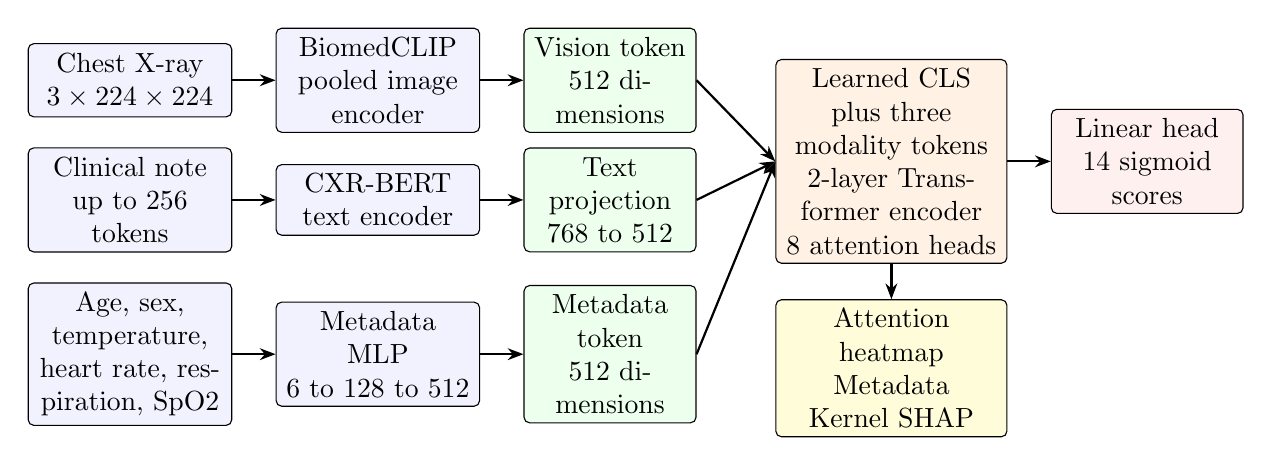
\begin{tikzpicture}[
  node distance=0.55cm and 0.55cm,
  block/.style={draw, rounded corners=2pt, align=center, minimum height=0.85cm, text width=2.35cm, fill=blue!5},
  smallblock/.style={draw, rounded corners=2pt, align=center, minimum height=0.75cm, text width=1.95cm, fill=green!7},
  arr/.style={-{Stealth[length=2mm]}, thick}
]
\node[block] (image) {Chest X-ray\\$3\times224\times224$};
\node[block, right=of image] (vision) {BiomedCLIP\\pooled image encoder};
\node[smallblock, right=of vision] (vfeat) {Vision token\\512 dimensions};
\node[block, below=0.38cm of image] (note) {Clinical note\\up to 256 tokens};
\node[block, right=of note] (text) {CXR-BERT\\text encoder};
\node[smallblock, right=of text] (tfeat) {Text projection\\768 to 512};
\node[block, below=0.38cm of note] (meta) {Age, sex, temperature,\\heart rate, respiration, SpO2};
\node[block, right=of meta] (mlp) {Metadata MLP\\6 to 128 to 512};
\node[smallblock, right=of mlp] (mfeat) {Metadata token\\512 dimensions};
\node[block, right=1.0cm of vfeat, yshift=-1.03cm, text width=2.7cm, minimum height=1.25cm, fill=orange!10] (fusion) {Learned CLS plus three modality tokens\\2-layer Transformer encoder\\8 attention heads};
\node[block, right=of fusion, text width=2.2cm, fill=red!6] (head) {Linear head\\14 sigmoid scores};
\node[smallblock, below=0.45cm of fusion, text width=2.7cm, fill=yellow!15] (xai) {Attention heatmap\\Metadata Kernel SHAP};
\draw[arr] (image) -- (vision);
\draw[arr] (vision) -- (vfeat);
\draw[arr] (note) -- (text);
\draw[arr] (text) -- (tfeat);
\draw[arr] (meta) -- (mlp);
\draw[arr] (mlp) -- (mfeat);
\draw[arr] (vfeat.east) -- (fusion.west);
\draw[arr] (tfeat.east) -- (fusion.west);
\draw[arr] (mfeat.east) -- (fusion.west);
\draw[arr] (fusion) -- (head);
\draw[arr] (fusion) -- (xai);
\end{tikzpicture}
\caption{Implemented X-Fusion inference path. The image branch supplies one pooled vector, and the fusion sequence contains a learned CLS token plus one token from each of the three modalities. The explainability outputs are post-hoc and do not establish clinical localization or causation.}
\label{fig:architecture}
\end{figure*}

\section{Methods}
\subsection{Inputs and Encoders}
The image is resized to 224 by 224 pixels, converted to RGB, and normalized using fixed channel-wise means and standard deviations. BiomedCLIP's image encoder returns a 512-dimensional pooled feature, which is represented as one token. Although a ViT internally processes patches, the fusion module in this implementation does not receive the individual patch tokens.

The clinical note is tokenized with truncation at 256 tokens and encoded by CXR-BERT. The first token representation is projected from the encoder hidden size, typically 768, to 512 dimensions using a learned linear layer. The six metadata inputs are ordered as age, sex, temperature, heart rate, respiratory rate, and oxygen saturation. A multilayer perceptron maps six values through a 128-unit hidden layer to 512 dimensions. The current model does not apply cohort-derived z-score normalization to these metadata values.

Let $I$ denote the preprocessed image, $T$ the tokenized note, and $m\in\mathbb{R}^{6}$ the metadata vector. The three encoder outputs are defined in \eqref{eq:encoders}:
\begin{align}
z_v &= f_{\mathrm{BiomedCLIP}}(I) \in \mathbb{R}^{512}, \\
z_t &= W_t h_{\mathrm{CLS}}^{\mathrm{CXR\text{-}BERT}}(T) \in \mathbb{R}^{512}, \\
u_m &= \operatorname{Dropout}(\operatorname{GELU}(W_1m+b_1)) \in \mathbb{R}^{128}, \\
z_m &= \operatorname{GELU}(W_2u_m+b_2) \in \mathbb{R}^{512}.
\label{eq:encoders}
\end{align}

\subsection{Transformer Fusion and Classification}
A learned 512-dimensional classification token is concatenated with the vision, text, and metadata tokens. The resulting sequence has four tokens and is processed by a two-layer, eight-head PyTorch Transformer encoder. This module performs self-attention over the four-token sequence; it is not a separately implemented patch-level cross-attention block. The final CLS representation is passed through dropout and a linear layer to produce fourteen logits. Independent sigmoid functions convert the logits to finding probabilities, allowing multiple findings to be predicted for one image.

The input sequence, scaled dot-product attention, and output probabilities are defined in \eqref{eq:fusion}:
\begin{align}
S_0 &= [e_{\mathrm{CLS}};z_v;z_t;z_m] \in \mathbb{R}^{4\times512}, \\
\operatorname{Attn}(Q,K,V) &=
\operatorname{softmax}\!\left(\frac{QK^{\mathsf T}}{\sqrt{d_k}}\right)V, \\
h &= \operatorname{Transformer}(S_0)_{\mathrm{CLS}}, \\
p_k &= \sigma((W_ch+b_c)_k),\quad k=1,\ldots,14.
\label{eq:fusion}
\end{align}

The output label set follows NIH ChestX-ray14: Atelectasis, Cardiomegaly, Effusion, Infiltration, Mass, Nodule, Pneumonia, Pneumothorax, Consolidation, Edema, Emphysema, Fibrosis, Pleural Thickening, and Hernia \cite{wang2017}.

\subsection{Training Objective}
The Lightning training wrapper combines Asymmetric Loss (ASL) with a symmetric image-text InfoNCE term. For a batch of size $B$, the implemented objective is given in \eqref{eq:objective}:
\begin{equation}
\mathcal{L}=\mathcal{L}_{\mathrm{ASL}}+0.1\mathcal{L}_{\mathrm{InfoNCE}}.
\label{eq:objective}
\end{equation}
For class $k$, the code clips easy negative probabilities using $p_{m,k}=\max(p_k-0.05,0)$ and uses
\begin{equation}
\begin{aligned}
\mathcal{L}_{\mathrm{ASL}}=-\frac{1}{B}\sum_{i=1}^{B}\sum_{k=1}^{14}\Big[&
y_{ik}(1-p_{ik})^{\gamma_+}\log p_{ik}\\
&+(1-y_{ik})p_{m,ik}^{\gamma_-}\log(1-p_{m,ik})\Big],
\end{aligned}
\label{eq:asl}
\end{equation}
where $\gamma_+=1$ and $\gamma_-=4$. The contrastive term normalizes the vision and text embeddings, forms the batch similarity matrix $s_{ij}=v_i^{\mathsf T}t_j/\tau$, and applies cross-entropy in both directions as shown in \eqref{eq:infonce}:
\begin{equation}
\mathcal{L}_{\mathrm{InfoNCE}}=\tfrac{1}{2}\left[
\operatorname{CE}(S,I_B)+\operatorname{CE}(S^{\mathsf T},I_B)\right],
\qquad \tau=0.07.
\label{eq:infonce}
\end{equation}
The optimizer is AdamW and the training module configures cosine annealing.

\subsection{Explainability Outputs}
The visual helper hooks the query-key-value projection in the final vision attention block, reconstructs attention scores, averages the CLS-to-patch attention over heads, reshapes the resulting 196 values to a 14 by 14 grid, and overlays the map on the image. This is an attention visualization. It does not use the target disease logit's gradient or compute layer-wise gradient-weighted attention rollout; therefore, we do not describe it as Chefer-CAM or Grad-CAM.

For metadata, Kernel SHAP varies the six input values while keeping image and text features fixed. The implementation takes absolute attribution magnitudes and aggregates them across all fourteen outputs before normalization. It therefore provides aggregate relative metadata importance, not signed per-disease contributions.

\section{Data and Training Protocol}
\subsection{Dataset Source and Splitting}
The data module reads the NIH ChestX-ray14 metadata CSV and the official train/validation and test image lists. It filters the CSV to image files available locally, then creates a validation partition by patient identifier from the official train/validation pool. The code sets a NumPy seed of 42 for this patient-level partition. Training images receive random flipping, rotation, brightness, and contrast augmentation; validation and test images use deterministic resizing and normalization.

The NIH ChestX-ray14 release contains 112,120 radiographs. In the local workspace, 31,877 PNG files were present, of which 31,630 matched entries in the metadata CSV. Applying the project's official image lists and patient-wise validation split yielded the counts in Table~\ref{tab:local_split}. The resulting subset is smaller than the full release and should not be described as a complete-benchmark evaluation.

\begin{table}[t]
\caption{Image and Patient Counts in the Local NIH Subset}
\label{tab:local_split}
\centering
\scriptsize
\begin{tabular}{lrr}
\toprule
Split & Images & Patients \\
\midrule
Training & 21,964 & 9,939 \\
Validation & 2,566 & 1,104 \\
Test & 7,100 & 1,137 \\
\midrule
Total & 31,630 & 12,180 \\
\bottomrule
\end{tabular}
\end{table}

The training and validation partitions are formed from the official train/validation list; the official test list supplies the test partition. The counts were obtained by running the repository's split logic against the local CSV and image files. Patient identifiers do not overlap across the three resulting partitions. The CSV supplies patient age and gender, while the auxiliary notes and several vital signs are generated rather than collected clinical observations.

\begin{figure}[t]
\centering
\includegraphics[width=\columnwidth]{../../backend/data/nih_cxr14/images/00000001_000.png}
\caption{Example local NIH ChestX-ray14 image. The accompanying CSV lists the image-level finding label as Cardiomegaly. The dataset label is weak supervision and is not an independent expert annotation for this figure.}
\label{fig:sample}
\end{figure}

\subsection{Synthetic Auxiliary Modalities and Leakage Risk}
The dataset implementation does not load real per-image radiology reports. It creates report-like text from each image's disease labels using templates. It also samples temperature, heart rate, respiratory rate, and oxygen saturation from distributions conditioned on the disease labels; age and sex are read from the CSV. These generated text and vital values directly encode information derived from the targets. This is target leakage and can make learned associations and evaluation results misleading. Further, random templates and vital values are generated when samples are read, so auxiliary inputs can vary between epochs and evaluation passes.

Accordingly, the current data pipeline is suitable for exercising the multimodal software path, but it does not establish that the model learned clinically valid independent signals from text and vital signs. Replacing the synthetic fields with genuinely paired, time-aligned clinical records is a prerequisite for a valid multimodal performance study.

\begin{figure*}[t]
\centering
\resizebox{\textwidth}{!}{%
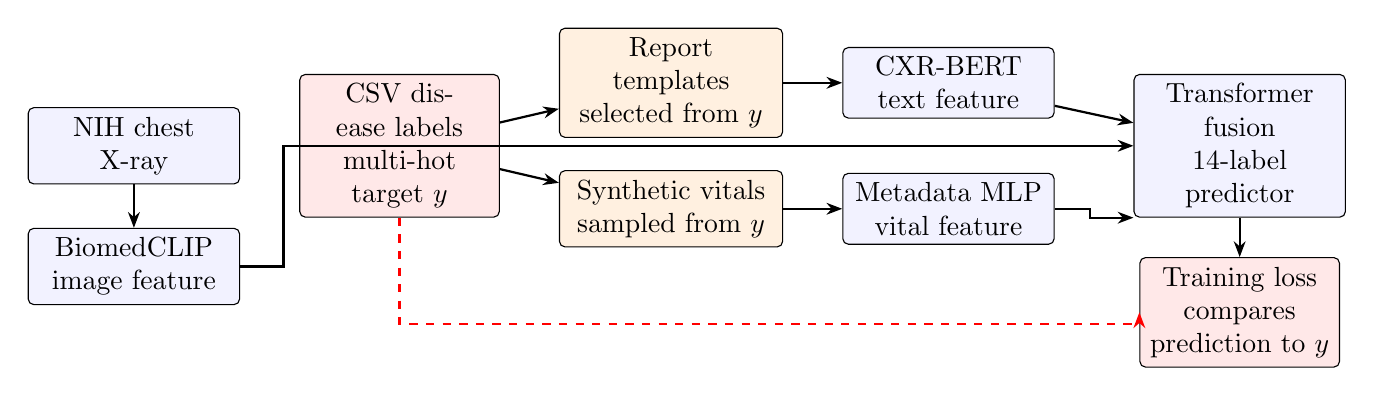
\begin{tikzpicture}[
  node distance=0.65cm and 0.75cm,
  box/.style={draw,rounded corners=2pt,align=center,minimum height=0.85cm,text width=2.45cm,fill=blue!5},
  gen/.style={draw,rounded corners=2pt,align=center,minimum height=0.85cm,text width=2.6cm,fill=orange!12},
  target/.style={draw,rounded corners=2pt,align=center,minimum height=0.85cm,text width=2.3cm,fill=red!9},
  flow/.style={-{Stealth[length=2mm]},thick},
  leak/.style={-{Stealth[length=2mm]},thick,dashed,red}
]
\node[box] (image) {NIH chest X-ray};
\node[target,right=of image] (label) {CSV disease labels\\multi-hot target $y$};
\node[box,below=0.55cm of image] (vision) {BiomedCLIP\\image feature};
\node[gen,right=of label,yshift=0.8cm] (report) {Report templates\\selected from $y$};
\node[gen,right=of label,yshift=-0.8cm] (vitals) {Synthetic vitals\\sampled from $y$};
\node[box,right=of report] (textenc) {CXR-BERT\\text feature};
\node[box,right=of vitals] (metaenc) {Metadata MLP\\vital feature};
\node[box,right=1.0cm of textenc,yshift=-0.8cm] (fusion) {Transformer fusion\\14-label predictor};
\node[target,below=0.5cm of fusion] (loss) {Training loss\\compares prediction to $y$};
\draw[flow] (image) -- (vision);
\draw[flow] (label) -- (report);
\draw[flow] (label) -- (vitals);
\draw[flow] (report) -- (textenc);
\draw[flow] (vitals) -- (metaenc);
\draw[flow] (vision.east) -- ++(0.55,0) |- (fusion.west);
\draw[flow] (textenc) -- (fusion);
\draw[flow] (metaenc.east) -- ++(0.45,0) |- (fusion.south west);
\draw[flow] (fusion) -- (loss);
\draw[leak] (label.south) -- ++(0,-1.35) -| (loss.west);
\end{tikzpicture}
}%
\caption{Training data flow in the current dataset code. The dashed red path highlights target leakage: disease labels determine synthetic report text and vital distributions, while the same labels supervise the predictor.}
\label{fig:leakage}
\end{figure*}

\subsection{Configured Training Run}
The advanced laptop training script specifies a batch size of 4, 15 maximum epochs, gradient accumulation over 8 batches, mixed precision, learning rate $2\times10^{-4}$, and weight decay $10^{-4}$. A stored Lightning hyperparameter file records the same learning rate and weight decay, with the text encoder frozen and the vision encoder configured as unfrozen. The script attempts to selectively unfreeze the final vision blocks by matching parameter-name substrings. Because this matching depends on the installed OpenCLIP model's parameter names, the exact set of trainable vision parameters should be verified before reproducing or reporting that run.

\begin{table}[t]
\caption{Implementation Configuration Recorded in the Repository}
\label{tab:config}
\centering
\scriptsize
\begin{tabular}{p{0.25\columnwidth}p{0.60\columnwidth}}
\toprule
Component & Repository configuration \\
\midrule
Image input & RGB, resized to $224\times224$ \\
Image encoder & BiomedCLIP pooled feature, 512 dimensions \\
Text encoder & CXR-BERT CLS projection, 768 to 512 \\
Metadata encoder & MLP, 6 to 128 to 512 \\
Fusion & 4 tokens; 2 Transformer layers; 8 heads \\
Output & 14 independent sigmoid scores \\
Loss & ASL plus 0.1 times InfoNCE \\
Advanced run & Batch 4; up to 15 epochs; accumulation 8 \\
Optimizer & AdamW; cosine annealing scheduler \\
Serving device & CPU or CUDA selected at startup \\
\bottomrule
\end{tabular}
\end{table}

\section{System Implementation and Verification}
The backend is implemented with FastAPI and Uvicorn. At startup, it constructs the model and loads a compatible checkpoint from the backend checkpoint directory. The prediction endpoint accepts a JPEG, PNG, or WebP image, a note, and a JSON metadata object. It returns the sorted fourteen-class probabilities, a primary score, an attention image, and metadata attribution values when SHAP succeeds. The frontend is implemented with Next.js, React, and TypeScript; it provides image upload, sample cases, form validation, result visualization, and session-only history.

A runtime smoke check recorded in the development session loaded the checkpoint, returned HTTP 200 from the health endpoint, and returned HTTP 200 for two prediction requests. This verifies that the local request path can execute; it is not a test-set evaluation and does not establish model accuracy, calibration, clinical utility, or latency.

\begin{table}[t]
\caption{Observed Local Software Smoke Checks}
\label{tab:smoke}
\centering
\scriptsize
\begin{tabular}{p{0.34\columnwidth}p{0.16\columnwidth}p{0.28\columnwidth}}
\toprule
Check & Observed & Interpretation \\
\midrule
Backend health & HTTP 200 & Checkpoint loaded \\
Prediction requests & 2 received HTTP 200 & API path executed \\
Frontend root page & HTTP 200 & UI served successfully \\
\bottomrule
\end{tabular}
\end{table}

\section{Results and Limitations}
The saved Lightning event log contains fourteen epoch-level records from the advanced local run. Figure~\ref{fig:training_trace} plots the logged training objective and validation classification loss as separate traces. The training objective fell from 0.1545 to 0.1190; the validation loss fell from 0.0207 to 0.0007. These are values recorded by the project, not reconstructed or illustrative data. The training objective includes the InfoNCE term, whereas validation loss is the classification loss alone, so the two curves should not be compared directly.

\begin{figure}[t]
\centering
\includegraphics[width=\columnwidth]{../../paper_assets/fig4_training_trace.png}
\caption{Training and validation losses logged over fourteen epochs in the saved advanced run. The training objective includes ASL and InfoNCE; validation loss includes ASL only. Because auxiliary inputs are generated from disease labels, this is an optimization trace and not evidence of generalization or clinical performance.}
\label{fig:training_trace}
\end{figure}

The repository does not contain a reproducible test-prediction file, per-class metric output, calibrated thresholds, or auditable ROC/AUPRC evaluation artifacts. The validation metrics in the event log are also affected by label-derived notes and vital signs. Earlier draft material included disease-level scores and ROC/ablation graphics, but their provenance could not be verified from the executable code or available artifacts; those results are omitted. No benchmark performance claim is made.

The main limitation is target leakage through the generated text and vital signs. Other limitations include incomplete local image availability, stochastic synthetic inputs, no metadata normalization, a pooled image vector rather than patch-token fusion, unverified selective fine-tuning behavior, and no external or prospective clinical validation. The attention map and aggregate SHAP values are aids for inspecting model outputs; they do not establish lesion localization or causal clinical reasoning. X-Fusion is a research prototype, not a medical device, and should not be used to guide patient care.

\section{Future Work}
Future development should first replace label-derived text and vitals with real, independently collected, properly linked clinical data, while recording missingness and acquisition times. A reproducible evaluation pipeline should save predictions and report per-class AUROC, AUPRC, sensitivity, specificity, calibration, and confidence intervals on patient-disjoint test data. The training code should log and verify the exact trainable parameter names and normalize continuous metadata using training-only statistics. Additional work includes a validated missing-modality strategy, clinically appropriate threshold calibration, external-site validation, DICOM input support, privacy and security controls, and clinician-reviewed evaluation of explanations.

\section{Conclusion}
X-Fusion demonstrates an end-to-end software prototype for combining chest radiographs, clinical notes, and structured patient values. Its implementation connects pretrained medical encoders, a metadata MLP, four-token Transformer fusion, multi-label outputs, post-hoc explanations, a FastAPI service, and a Next.js interface. The project currently supports technical workflow demonstration, not a clinically validated performance claim. Reliable multimodal evaluation depends on replacing label-derived auxiliary inputs and producing reproducible patient-level test evidence.

\section*{Acknowledgment}
The authors thank K. Vishal Reddy for mentorship and project guidance. The NIH ChestX-ray14 dataset is acknowledged as the intended image benchmark. This manuscript does not claim that the other datasets mentioned in earlier drafts were used in the implementation described here.

\begin{thebibliography}{00}
\bibitem{wang2017}
X. Wang, Y. Peng, L. Lu, Z. Lu, M. Bagheri, and R. M. Summers, ``ChestX-ray8: Hospital-scale chest X-ray database and benchmarks on weakly-supervised classification and localization of common thorax diseases,'' in \emph{Proc. IEEE Conf. Comput. Vis. Pattern Recognit.}, 2017, pp. 2097--2106. [Online]. Available: \href{https://doi.org/10.1109/CVPR.2017.369}{doi:10.1109/CVPR.2017.369}

\bibitem{irvin2019}
J. Irvin \emph{et al.}, ``CheXpert: A large chest radiograph dataset with uncertainty labels and expert comparison,'' in \emph{Proc. AAAI Conf. Artif. Intell.}, vol. 33, 2019, pp. 590--597. [Online]. Available: \href{https://doi.org/10.1609/aaai.v33i01.3301590}{doi:10.1609/aaai.v33i01.3301590}

\bibitem{dosovitskiy2021}
A. Dosovitskiy \emph{et al.}, ``An image is worth 16x16 words: Transformers for image recognition at scale,'' in \emph{Proc. Int. Conf. Learn. Represent.}, 2021. [Online]. Available: \href{https://arxiv.org/abs/2010.11929}{arXiv:2010.11929}

\bibitem{biomedclip2023}
S. Zhang \emph{et al.}, ``BiomedCLIP: A multimodal biomedical foundation model pretrained on fifteen million scientific image-text pairs,'' arXiv:2303.00915, 2023. [Online]. Available: \href{https://arxiv.org/abs/2303.00915}{arXiv:2303.00915}

\bibitem{cxrbert2022}
B. Boecking \emph{et al.}, ``Making the most of text semantics to improve biomedical vision-language models,'' in \emph{Computer Vision -- ECCV 2022}, 2022. [Online]. Available: \href{https://arxiv.org/abs/2204.09817}{arXiv:2204.09817}

\bibitem{ridnik2021}
T. Ridnik, E. Ben-Baruch, A. Noy, and L. Zelnik-Manor, ``Asymmetric loss for multi-label classification,'' in \emph{Proc. IEEE/CVF Int. Conf. Comput. Vis.}, 2021, pp. 82--91. [Online]. Available: \href{https://doi.org/10.1109/ICCV48922.2021.00014}{doi:10.1109/ICCV48922.2021.00014}

\bibitem{oord2018}
A. van den Oord, Y. Li, and O. Vinyals, ``Representation learning with contrastive predictive coding,'' 2018. [Online]. Available: \href{https://arxiv.org/abs/1807.03748}{arXiv:1807.03748}

\bibitem{lundberg2017}
S. M. Lundberg and S.-I. Lee, ``A unified approach to interpreting model predictions,'' in \emph{Advances in Neural Information Processing Systems}, vol. 30, 2017. [Online]. Available: \href{https://papers.nips.cc/paper/7062-a-unified-approach-to-interpreting-model-predictions}{NeurIPS paper}

\bibitem{chefer2021}
H. Chefer, S. Gur, and L. Wolf, ``Transformer interpretability beyond attention visualization,'' in \emph{Proc. IEEE/CVF Conf. Comput. Vis. Pattern Recognit.}, 2021, pp. 782--791. [Online]. Available: \href{https://doi.org/10.1109/CVPR46437.2021.00084}{doi:10.1109/CVPR46437.2021.00084}

\bibitem{nihdataset}
National Institutes of Health Clinical Center, ``ChestX-ray14 dataset.'' [Online]. Available: \href{https://nihcc.app.box.com/v/ChestXray-Nihcc}{NIH dataset page}

\bibitem{davit2025}
M. Fu, C. Tantithamthavorn, and T. Le, ``DAViT: A domain-adapted vision transformer for automated pneumonia detection and explanation using chest X-ray images,'' \emph{IEEE Access}, vol. 13, pp. 103033--103044, 2025. [Online]. Available: \href{https://doi.org/10.1109/ACCESS.2025.3579314}{doi:10.1109/ACCESS.2025.3579314}

\end{thebibliography}

\end{document}
